\section{Light Sources}
{\color{blue} edited on 15 May by Benno\\
edited ... by ...}\\
This section is devoted to light sources for 3G IFOs. It includes the pre-stabilized high power lasers (PSL) and the squeezed light sources. It does NOT include filter cavities for frequency dependent squeezing quadrature rotation. 
\subsection{Current State of the Art}
\begin{itemize}
\item all advanced GWDs have problems with their lasers
\item several solutions are being tested: 200\,W class fiber amplifiers (AEI/LZH, MIT, Artemis) and coherently combined solid state amplifiers (AEI)
\item high power lasers demonstrated in lab
	\begin{itemize}
    \item 1064\,nm
    \item 1550\,nm
    \item $\rm 2\,\mu m$
	\end{itemize}
\item problem with durability
\item squeezed light sources 
\begin{itemize}
    \item 1064\,nm
    \item 1550\,nm
    \item $\rm 2\,\mu m$
	\end{itemize}
\end{itemize}

\subsection{Requirements and current/planned R\&D}
We analyzed available documentation and presentations on next generation gravitational wave detectors (GWDs) to extract requirements for the high power lasers and squeezers. In parallel the  R\&D currently performed within the worldwide gravitational wave (GW) community was identified by sending a questionnaire to 32 laser and sqeezing experts in all GW projects. The questionnaire asked for current and planned R\&D and for desired collaboration topics and coordination mechanisms. The findings are summarized in this sub section.
The requirements on the pre-stabilized high power laser and the squeezed light sources for 3rd generation GWDs do not seem to be well defined yet. The design of the Einstein Telescope (ET) as defined in the ET design study is build on a 500\,W laser at 1064\,nm in the spatial $\rm LG_{33}$ mode and a 3\,W laser at a wavelength of 1150\,nm in the fundamental Gaussian mode. Even though these are clear requirement, the ET design is currently re-evaluated. In particular the operation of the ET high power IFO in the spatial $\rm LG_{33}$ seems questionable. The current Cosmic Explore (CE) and LIGO Voyager (LV) designs are build on high power light sources with a power of 200\,W and a wavelength of 1550nm or longer for a small absorption coefficients for the light to be transmitted by Silicon test masses. The wavelength choice depends on several factors as e.g. available high power lasers, absorption of the bulk and the high reflective coatings of the test masses, scattering and the availability of photo detectors with high quantum efficiency. As information on several of these factors is missing, a final wavelength choice can not yet be made. Currently the wavelength of 1550\,nm and around $\rm 2\, \mu m $ are favored due to promising high power laser concepts for these wavelength. Hence R\&D on high power laser and squeezer for three different wavelength (1064\,nm, 1550\,nm and around $\rm 2\, \mu m $) has to be performed until the final operation wavelength are selected. All current 3G GWD designs are currently build on 10dB detected squeezing such that squeezed vacuum sources with squeezing levels of $> 15\,dB$ are required. No information on PSLs stability requirements for 3G GWD detectors could be found. As a 10 times better sensitivity is aimed for we assume that the power, frequency and beam jitter stability has to be a factor of 10 higher. Concerning the spatial and polarization purity we expect similar requirements as for the Advanced GWDs.
With the afore mentioned questionnaire we found, that the current or planned research of at least two groups covers the identified required research areas (see Fig. 
\begin{figure}[h]
% \centering
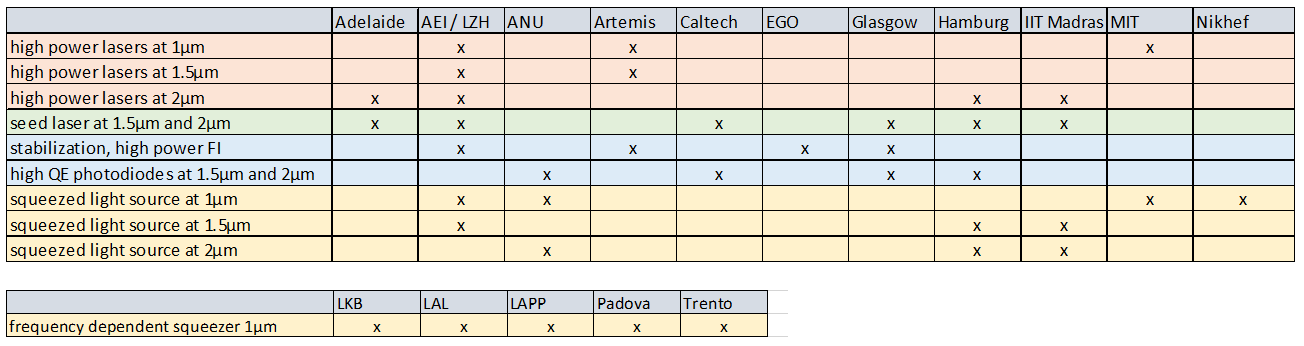
\includegraphics[scale=0.5]{Light_source_Fig1.png}
\caption{Current or planned R\&D on high power laser and squeezed vacuum sources}
\label{fig:LightSourceRD}
\end{figure}

% \subsubsection{3G initial}
% \subsubsection{future}
\subsection{Pathways and required facilities}
\subsubsection{laboratory prototypes}
Show that high power generation concepts works reliable, accept poor noise performance, missing diagnostic and actuators for stabilization
\subsubsection*{1064\,nm}
we assume reliability problem of 200\,W class fiber amplifier will be solved for Advanced detectors (current work at AEI/LZH, MIT and Artemis)\\
develop coherent combination techniques at 2x250W power level
\subsubsection*{1550\,nm}
assume AEI/LZH fiber amplifier development is successful
\subsubsection*{$\rm \bf 2\,\mu m$}
assume either Adelaide cryo HM or wavelength doubling of 1064\,nm in OPA is successful
\subsubsection*{stabilization}
develop stabilization concepts for all three wavelength adequate for free running noise and available actuators of laboratory PT developments
\subsubsection{engineering prototype}
after final wavelength selection transfer concepts to laser lab or company capable of designing and fabricating an engineering prototype that meets all requirements concerning power, noise performance, spatial and polarization purity, actuators with sufficient range and bandwidth, diagnostic\\
transfer engineering prototype to research lab for characterization and pre-stabilization\\
build several engineering prototypes for long-term/reliability tests
\subsection{Type of collaboration required:  small/large}
small, summarize results of questionnaire\\
once at engineering PT stage: synergy between projects requiring similar lasers (if possible avoid single supplier problem)

\subsection{Suggested mechanisms}
annual meetings, keep list of who does what,\\
team up of GWD projects and funding agencies in engineering PT stage
\subsection{Impact/relation to 2G and upgrades}
at 1064nm laser development for 2G and upgrades is in direct path to 3G and will serve as long-term test of some concepts